
\section{System Implementation} \label{sec:asasel:demo}
	
The ASASEL system was developed on the Java platform. Workflows are entered textually via a GUI illustrated in Figure \ref{fig:asaselGUI}. For a given ASASEL service coordination, the GUI (relying on the JGraph\footnote{http://www.jgraph.com/} library) provides the user a workflow visualization. Data services are represented in yellow whereas computation services are represented in blue, both with their corresponding labels.

The enactment of a workflow is enabled by two main components. First, a scheduler determines which service is executed at a given time according to a predefined policy. Second, composite services are executed by an interpreter that implements the full ASASEL language. Computation service workflows can also be visualized through the GUI, as shown at the right part of the screenshot in Figure \ref{fig:asaselGUI}. The interpreter was developed using the ANTLR\footnote{http://www.antlr.org/} parser generator.
	
During the execution of a workflow, data flows from the data services to several computation services via queues, as determined by the ASASEL specification. Computation services can be specified to output data in textual form in the GUI or to transmit it to another application. For instance, in our example application we output as a result data stream that denotes the tuples that are added and the tuples that are removed from the result dataset.
	
We developed a set of basic computation services that are used to build the operations for our example application. These services run on a Tomcat container supported by the JAX-WS reference implementation \footnote{https://jax-ws.dev.java.net/}, which enables to create stateful services.
	
Additionally, we implemented two test scenarios and their corresponding data services to use with our computation services. The first one is the location-based application introduced in Section \ref{sec:serviceOrientedWorkflows}. The second scenario is an adaptation of the online auctions NEXMark benchmark\footnote{http://datalab.cs.pdx.edu/niagara/NEXMark/} for XML stream query processing which we employed to obtain performance measurements. In brief, the measurements indicated a tolerable overhead for the use of services, which we consider outweighed by the advantages.
	
	%\begin{figure*}
	%	\centering
	%	\epsfig{file=Images/ASASEL.eps, scale=0.37}
	%	\caption{}
	%	\label{fig:asaselGUI}
	%\end{figure*}
	
	\begin{figure}
   \begin{center}
 %     \scalebox{0.675}{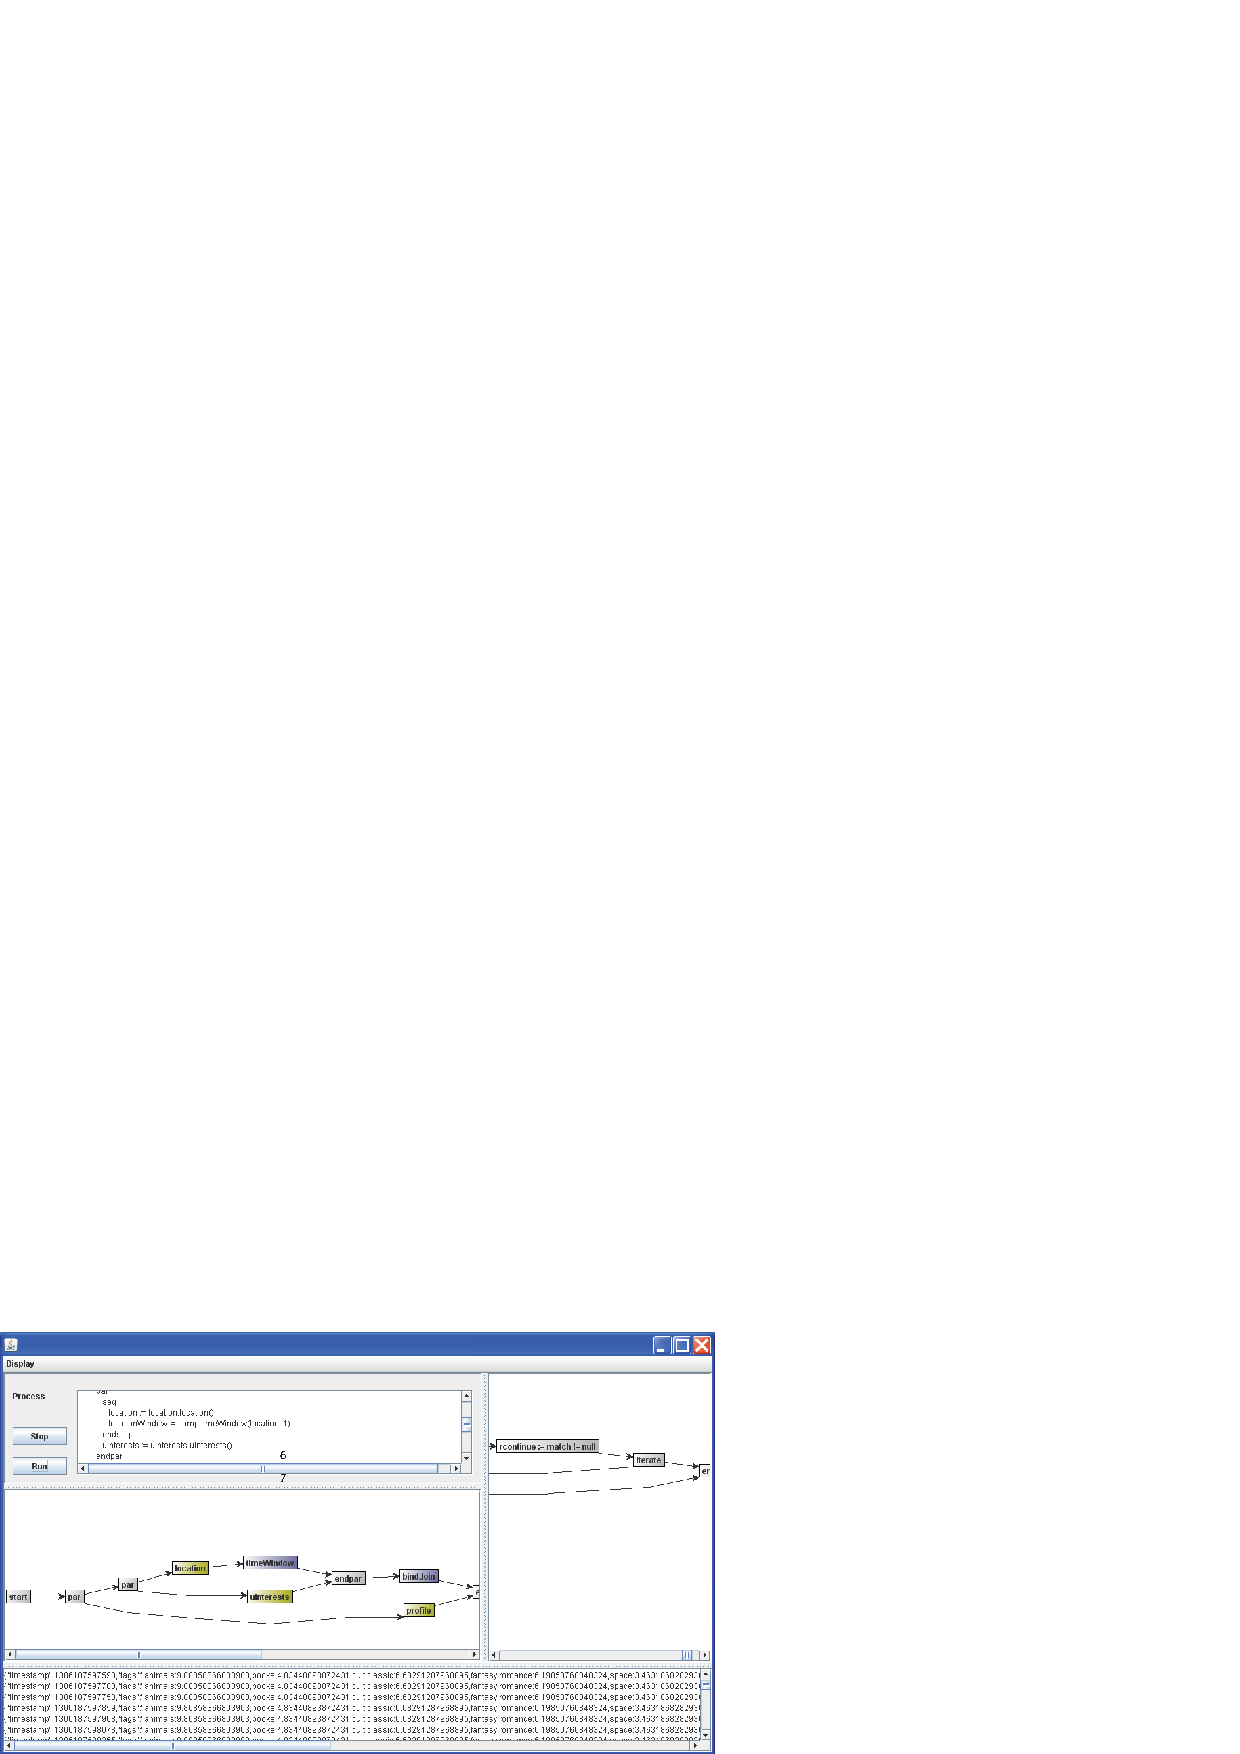
\includegraphics[natwidth=12.31cm,natheight=7.16cm]{Images/asaselgui.pdf}}
   \end{center}
   \caption{Caption of the ASASEL GUI}
   \label{fig:asaselGUI}
\end{figure}

